\section{Results and Discussion}
\label{sec:Results-and-Discussion}
As mentioned earlier, this section serves to present a graphical illustration of the results relevant to the experiments outlined in Section \ref{sec:Methodology} alongside a brief discussion.

\subsection{Experiment 1}
\label{subsec:Results-and-Discussion:Experiment-1}
The first of our experiments explored the relationship between the number of cars on a square lattice. Notably, we examined whether the \gls{bml} traffic model would achieve a free-flowing state of traffic given that the total number of cars $(n)$ did not exceed the length of one of the sides of the aforementioned square lattice $\left(n \leq \frac{X}{2}\right)$. To ascertain this, we ran simulations using our implementation of the \gls{bml} traffic model under the set of hyperparameters listed in Section \ref{subsec:Methodology:Experiment-1} and averaged the results over a total of 10 runs. Figure \ref{fig:Experiment-1.1} denotes the (averaged) mean velocity for each simulation under varying values of $\rho$. We note that for values of $n$ where $n \sim \frac{N}{2}$, the system tends to consistently reach a velocity of 1 and a free-flowing state of traffic which is in line with the theory outlined by \citeauthor{Austin} in their paper. In accordance with their paper, we observe that, for values of  $n < \frac{1}{2}(N)$, regardless how the cars are distributed in our $N \times N$ lattice then there will always exist an empty arc (over the diagonals of the square lattice in question) of length at least 2, and so the system will self-organize to a velocity of 1 in a finite amount of iterations. In the interest of preserving time and preventing this paper from being overtly length, we direct the reader to the original paper, located \href{https://arxiv.org/pdf/math/0607759.pdf}{here}, to better understand how \citeauthor{Austin} came about to prove this proposition. 

\begin{figure}[H]
    \centering
    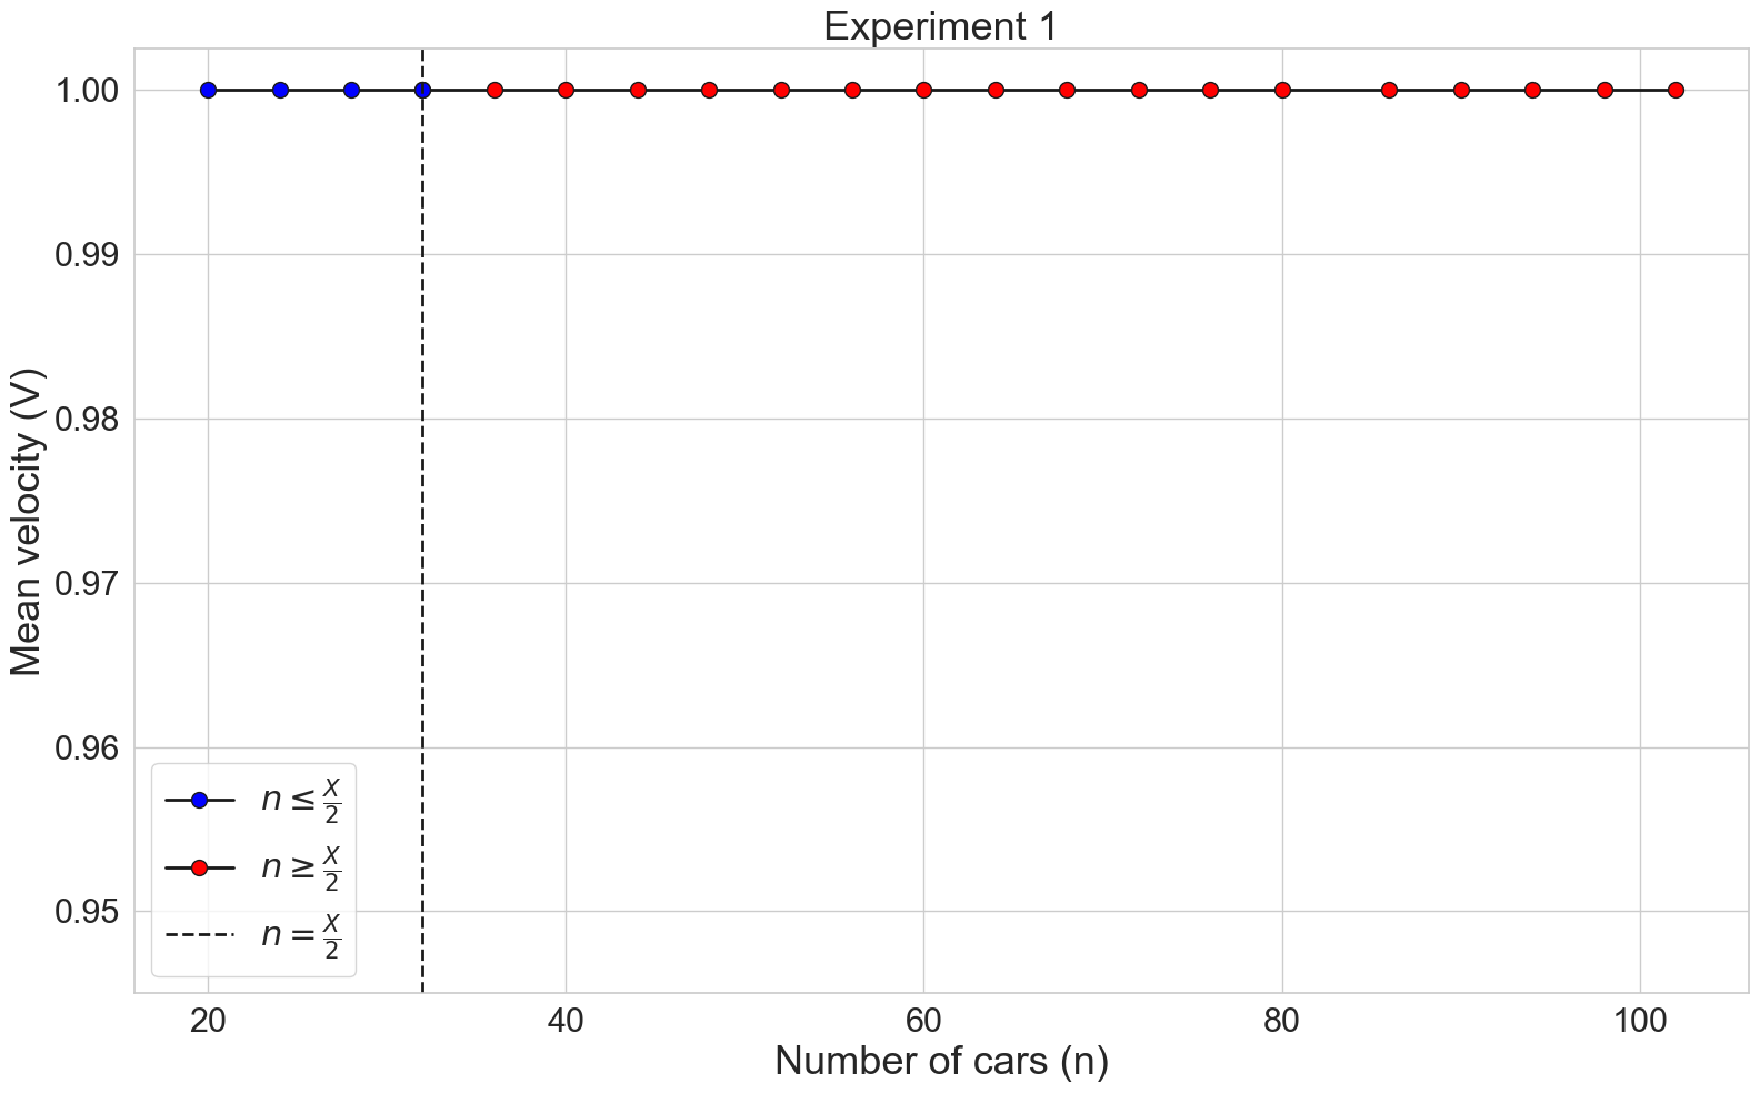
\includegraphics[width=\linewidth]{Images/Section 4/Experiment 1/1.2.pdf}
    \caption{Mean velocity of the simulations run under the set of hyperparameters pertaining to experiment 1. A mean velocity of $1.0$ denotes that the system experienced a smooth flow of traffic straight from the get-go and (in the worst case) experienced a number of collisions around the start.}
    \label{fig:Experiment-1.1}
\end{figure}

\subsection{Experiment 2}
\label{subsec:Results-and-Discussion:Experiment-2}
The results of experiment 2 are meant to ascertain that, as $\rho$ approaches 1, the \gls{bml} traffic model will reach a globally jammed phase, in which no car can make a move, infinitely often. To ascertain this, we ran we ran simulations using our implementation of the \gls{bml} traffic model under the set of hyperparameters listed in Section \ref{subsec:Methodology:Experiment-2}, and once again averaged the results over a total of 10 runs per value of $\rho$. Our findings are outlined in Figures \ref{fig:Experiment-2.1}, \ref{fig:Experiment-2.2}, \ref{fig:Experiment-2.3}, and \ref{fig:Experiment-2.4}. The basis of the arguments formulated by \citeauthor{Omer} revolve around the existence of blocking paths in configurations where $\rho > \rho_c$. To best understand this, take an initialization in which $\rho = 1:$  each and every car is immediately blocked by a car positioned directly in front of it and in this way no cars can make a move due to an infinite chain of blocking cars that define a set of \textit{"blocking paths"}. While this logic does not immediately extend to configurations in which $\rho < 1$, as such a chain will always be broken by an empty space, if we consider the previously defined network of blocking paths for a configuration at $\rho = 1$, then it is likely that these blocking paths still exist in systems configured at values of $\rho < 1$ (considering the fact that taking $\rho < 1$ is akin to removing a proportion of cars from a $\rho = 1$ configuration.) See Figure \ref{fig:Blocking-Paths-1} for an illustration.

\begin{figure}[H]
    \centering
    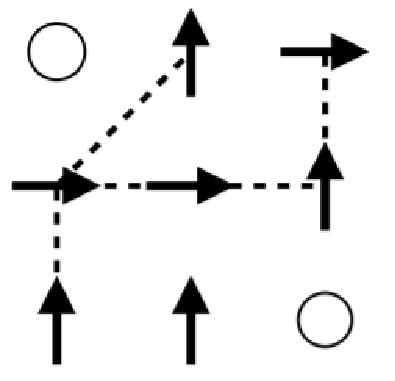
\includegraphics[width=0.475\linewidth]{Images/Section 4/Blocking-Paths-1.pdf}
    \caption{An illustration of blocking paths as per the findings of \citeauthor{Omer}.  Image source: \cite{Omer} licensed under \href{https://creativecommons.org/licenses/by/3.0/}{CC BY 3.0}.}
    \label{fig:Blocking-Paths-1}
\end{figure}

\begin{figure}[H]
    \centering
    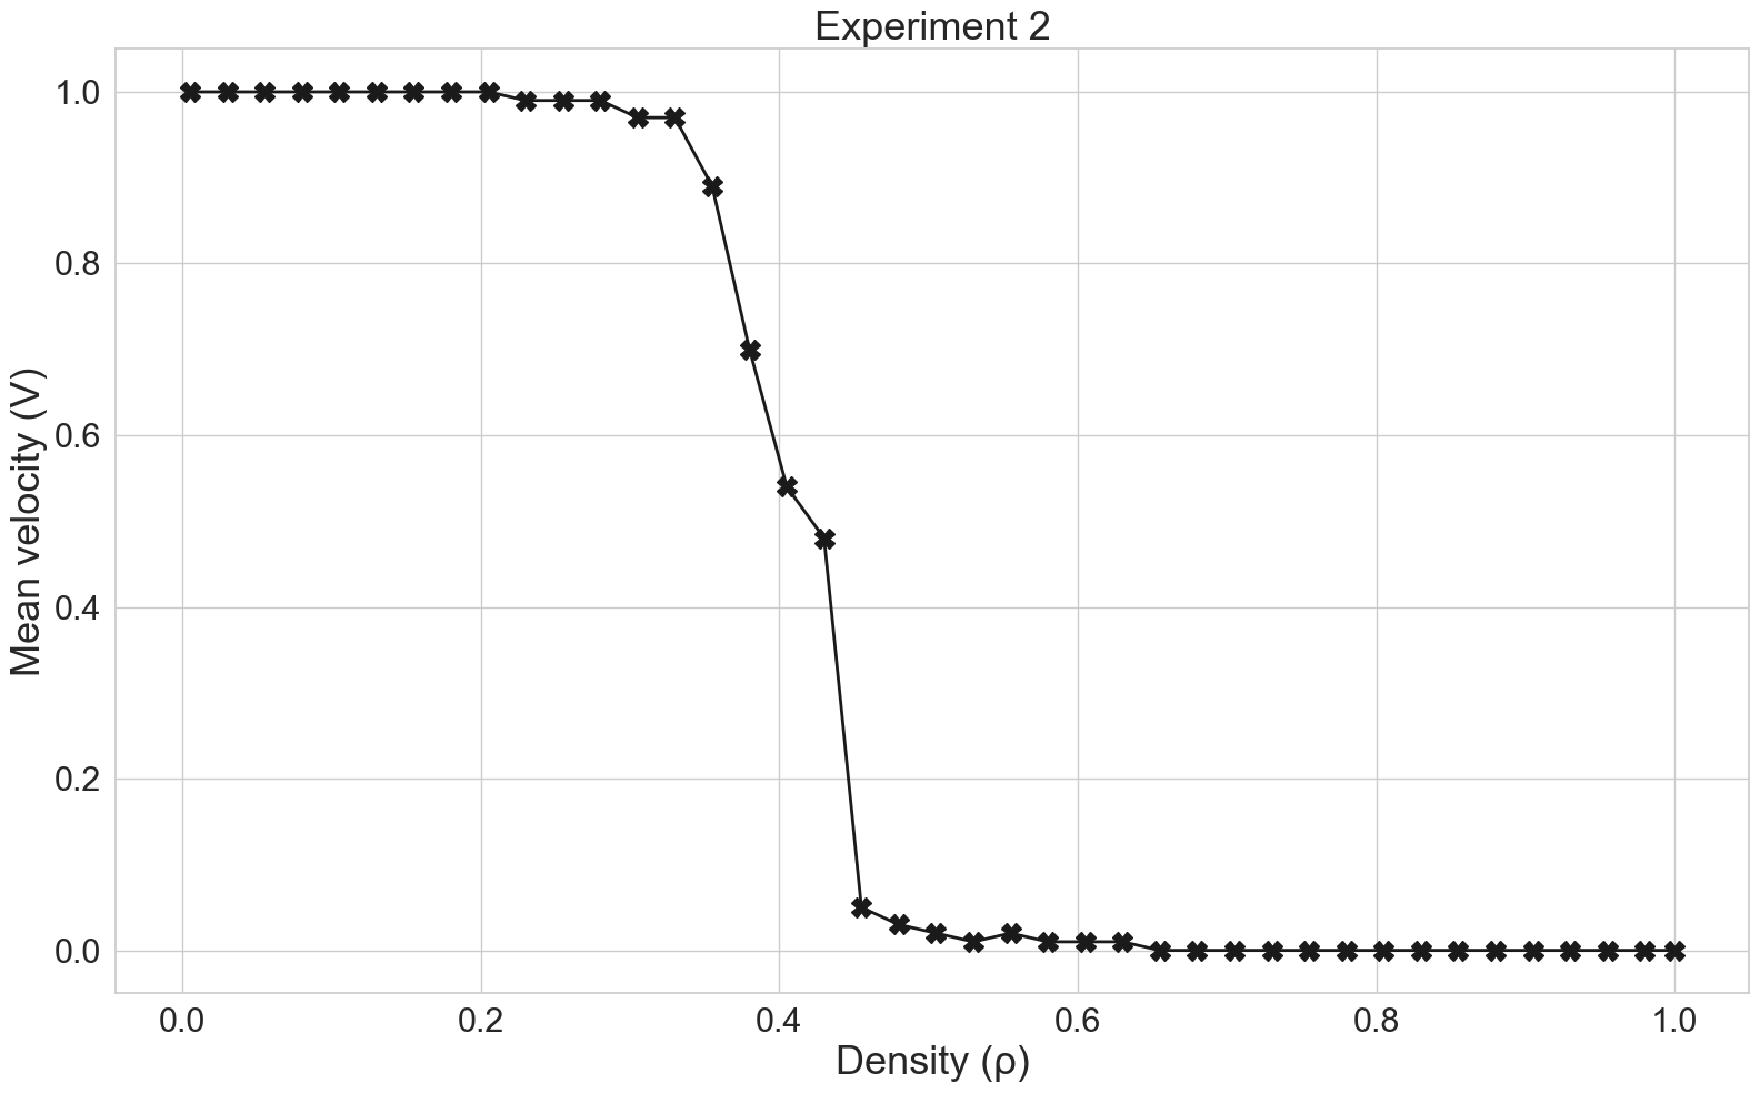
\includegraphics[width=\linewidth]{Images/Section 4/Experiment 2/2.1.pdf}
    \caption{Mean velocity per simulation averaged over a total of 10 runs per value of $\rho$.}
    \label{fig:Experiment-2.1}
\end{figure}

\vspace{3em}

\begin{figure}[H]
    \centering
    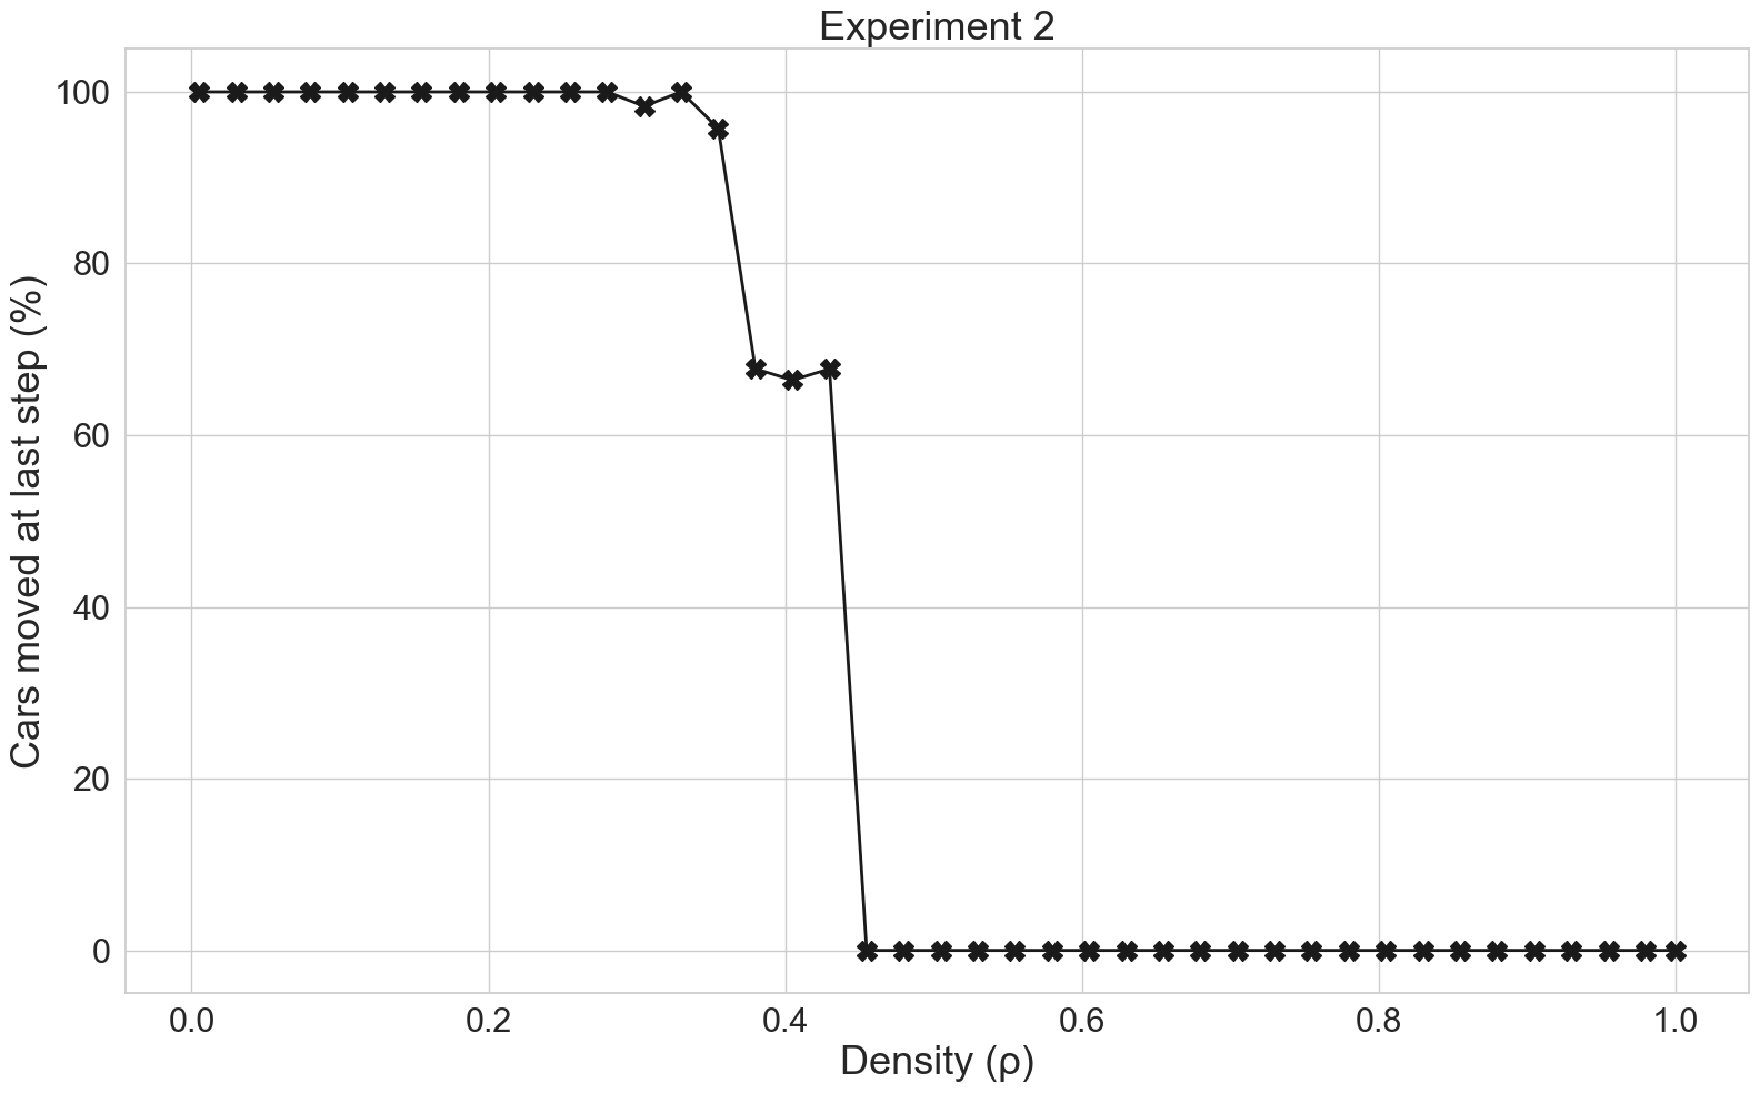
\includegraphics[width=\linewidth]{Images/Section 4/Experiment 2/2.2.pdf}
    \caption{Percentage of cars that moved at the last time step recorded for each of our simulations averaged over a total of 10 runs per value of $\rho$.}
    \label{fig:Experiment-2.2}
\end{figure}

\vspace{3em}

\begin{figure}[H]
    \centering
    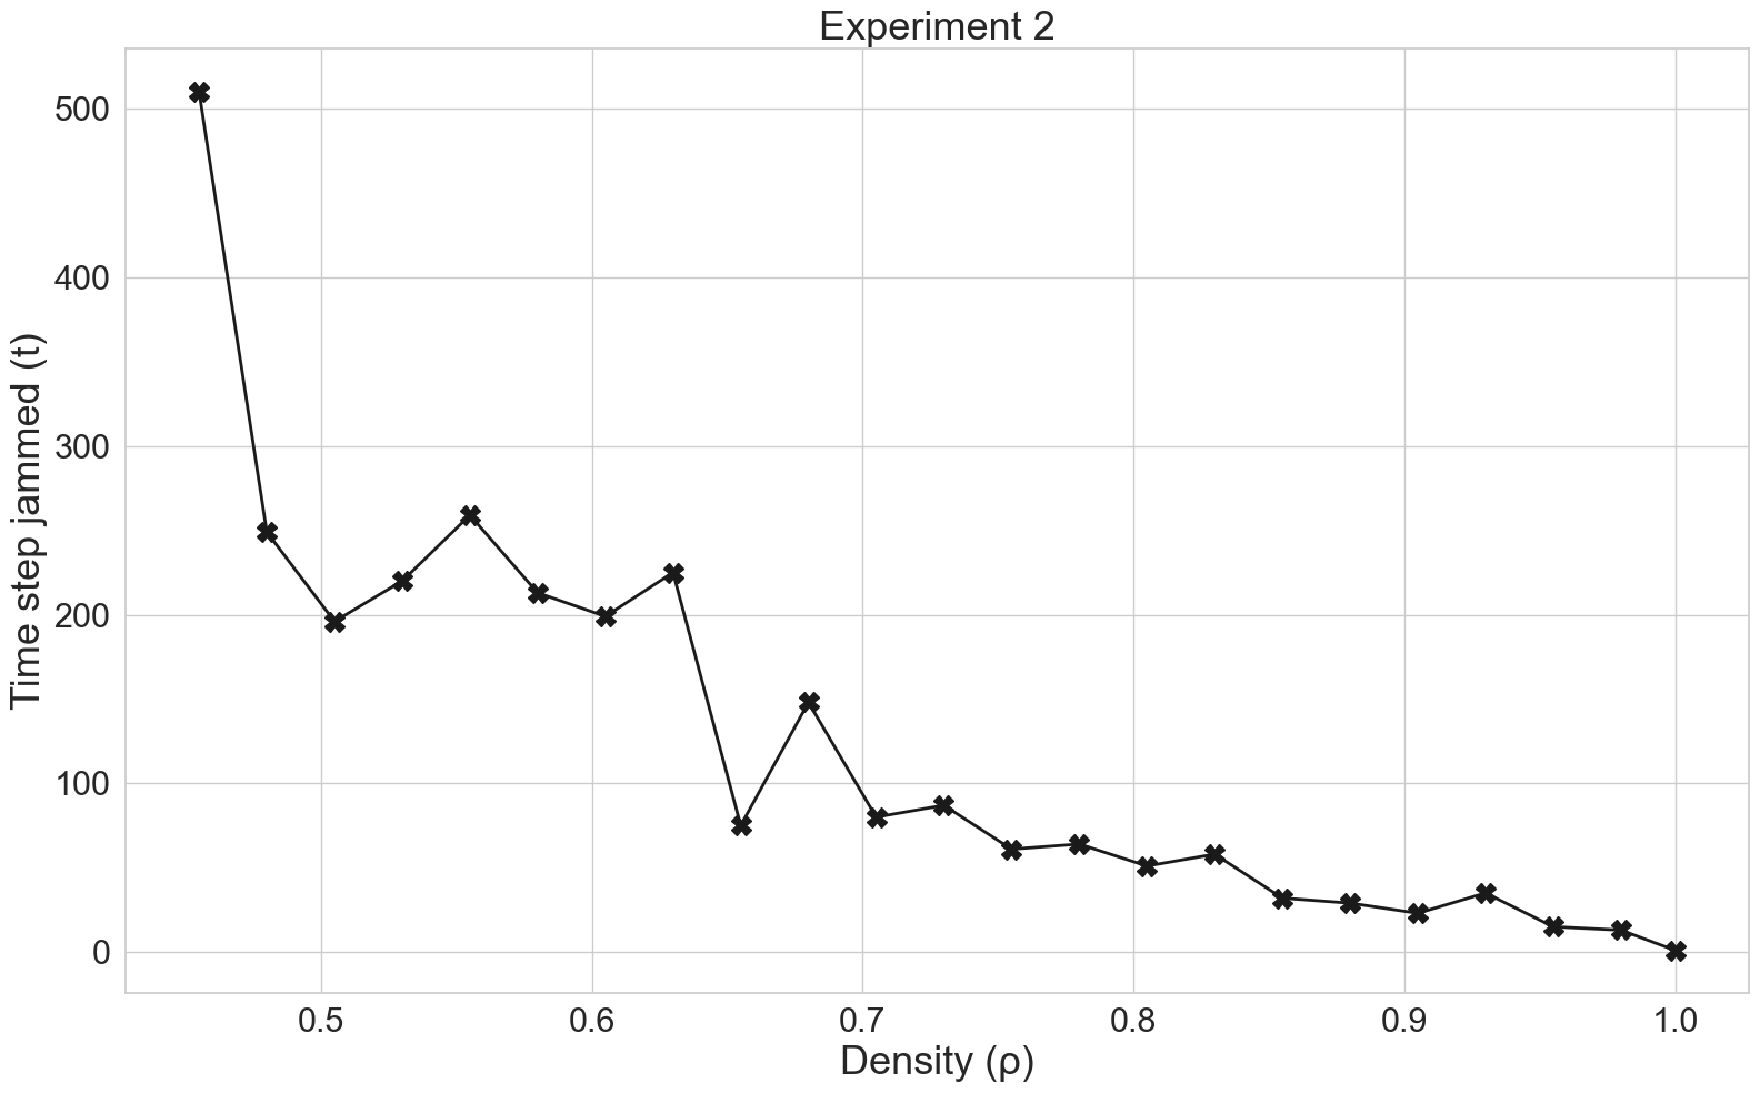
\includegraphics[width=\linewidth]{Images/Section 4/Experiment 2/2.3.pdf}
    \caption{Time step that the system jammed (if applicable) for each of our simulations averaged over a total of 10 runs per value of $\rho$.}
    \label{fig:Experiment-2.3}
\end{figure}

\vfill\null

\begin{figure}[H]
    \centering
    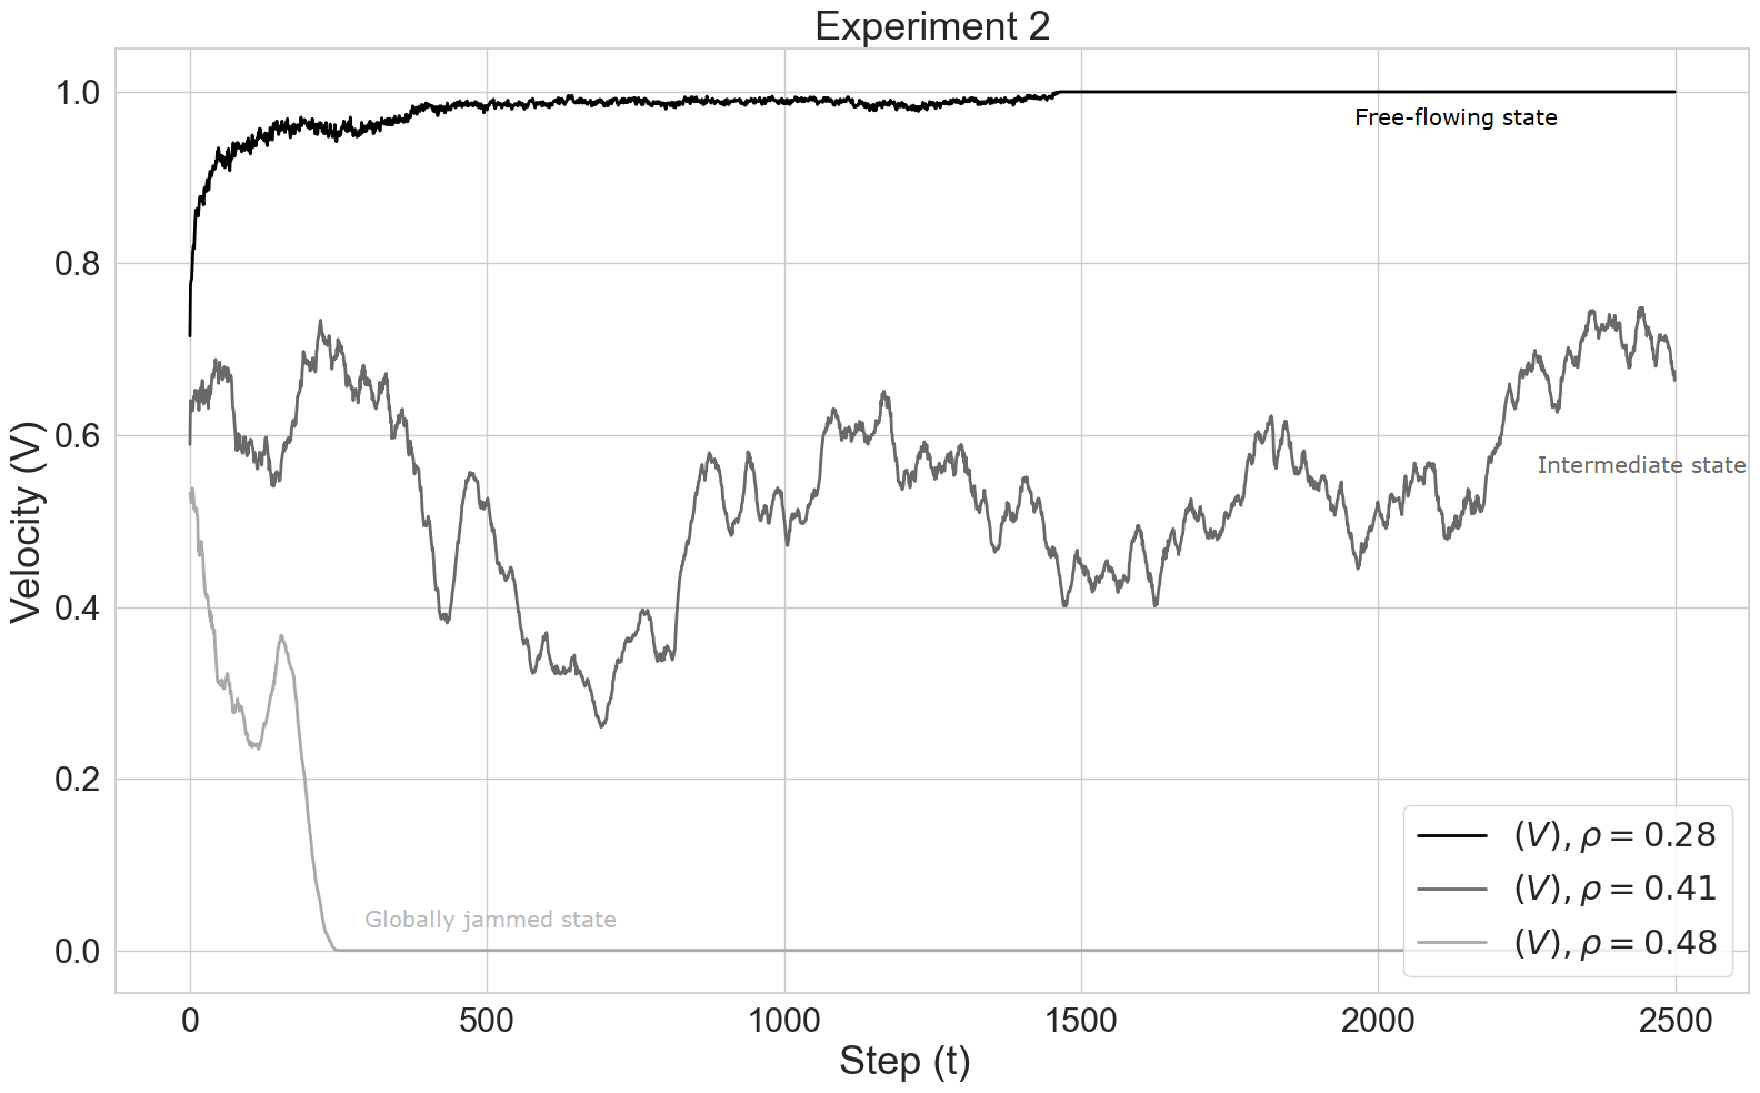
\includegraphics[width=\linewidth]{Images/Section 4/Experiment 2/2.4.pdf}
    \caption{A deeper look at the velocity per iteration of 3 different systems at 3 different densities that exhibit the different states of traffic flow associated with the \gls{bml} traffic model.}
    \label{fig:Experiment-2.4}
\end{figure}

\subsection{Experiment 3}
\label{subsec:Results-and-Discussion:Experiment-3}
The final experiment pertains to the emergence of periodic (with respect to time) intermediate states in the \gls{bml} traffic model that capture the essence of both the jammed state as well as the free-flowing state. In particular, the findings of \citeauthor{DSouza}, show that for a lattice of coprime dimensions and for values of $\rho \sim \rho_c$ the system will self-organize into periodic arrangements that consists of both jams as well as smoothly flowing traffic. To attempt to recreate this we initialized a $144 \times 89$ rectangular lattice with a density of $38\%$ and ran the simulation for a total of $7,500$ iterations. We noted the velocity per time step of the simulation and found that at around $t \sim 4,000$ the system self-organized to the previously defined intermediate state. The findings of our results can be seen in Figures \ref{fig:Experiment-3.1}, \ref{fig:Experiment-3.2}, and \ref{fig:Experiment-3.3}.

\begin{figure}[H]
    \centering
    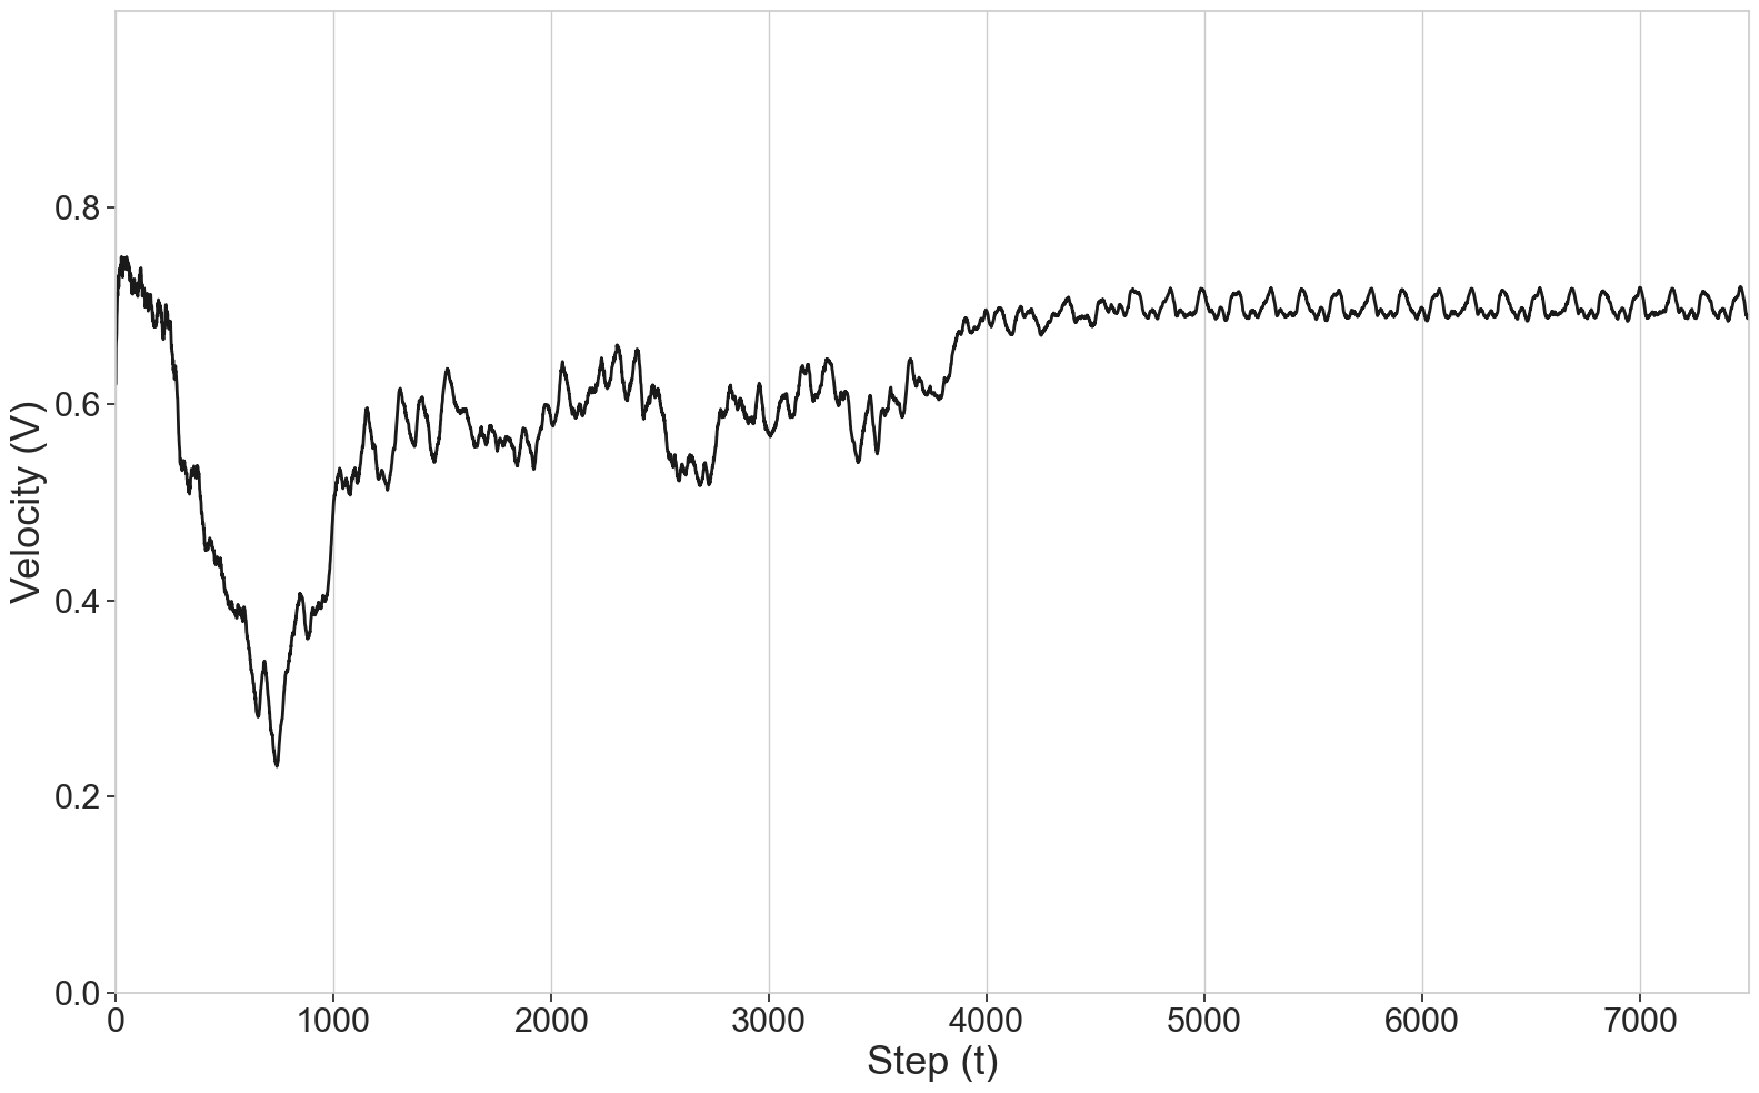
\includegraphics[width=\linewidth]{Images/Section 4/Experiment 3/Velocity.pdf}
    \caption{Velocity per time step of a simulation run on a rectangular lattice with coprime dimensions over a total of $7,500$ time steps.}
    \label{fig:Experiment-3.1}
\end{figure}

\vfill\null

\begin{figure}[H]
    \centering
    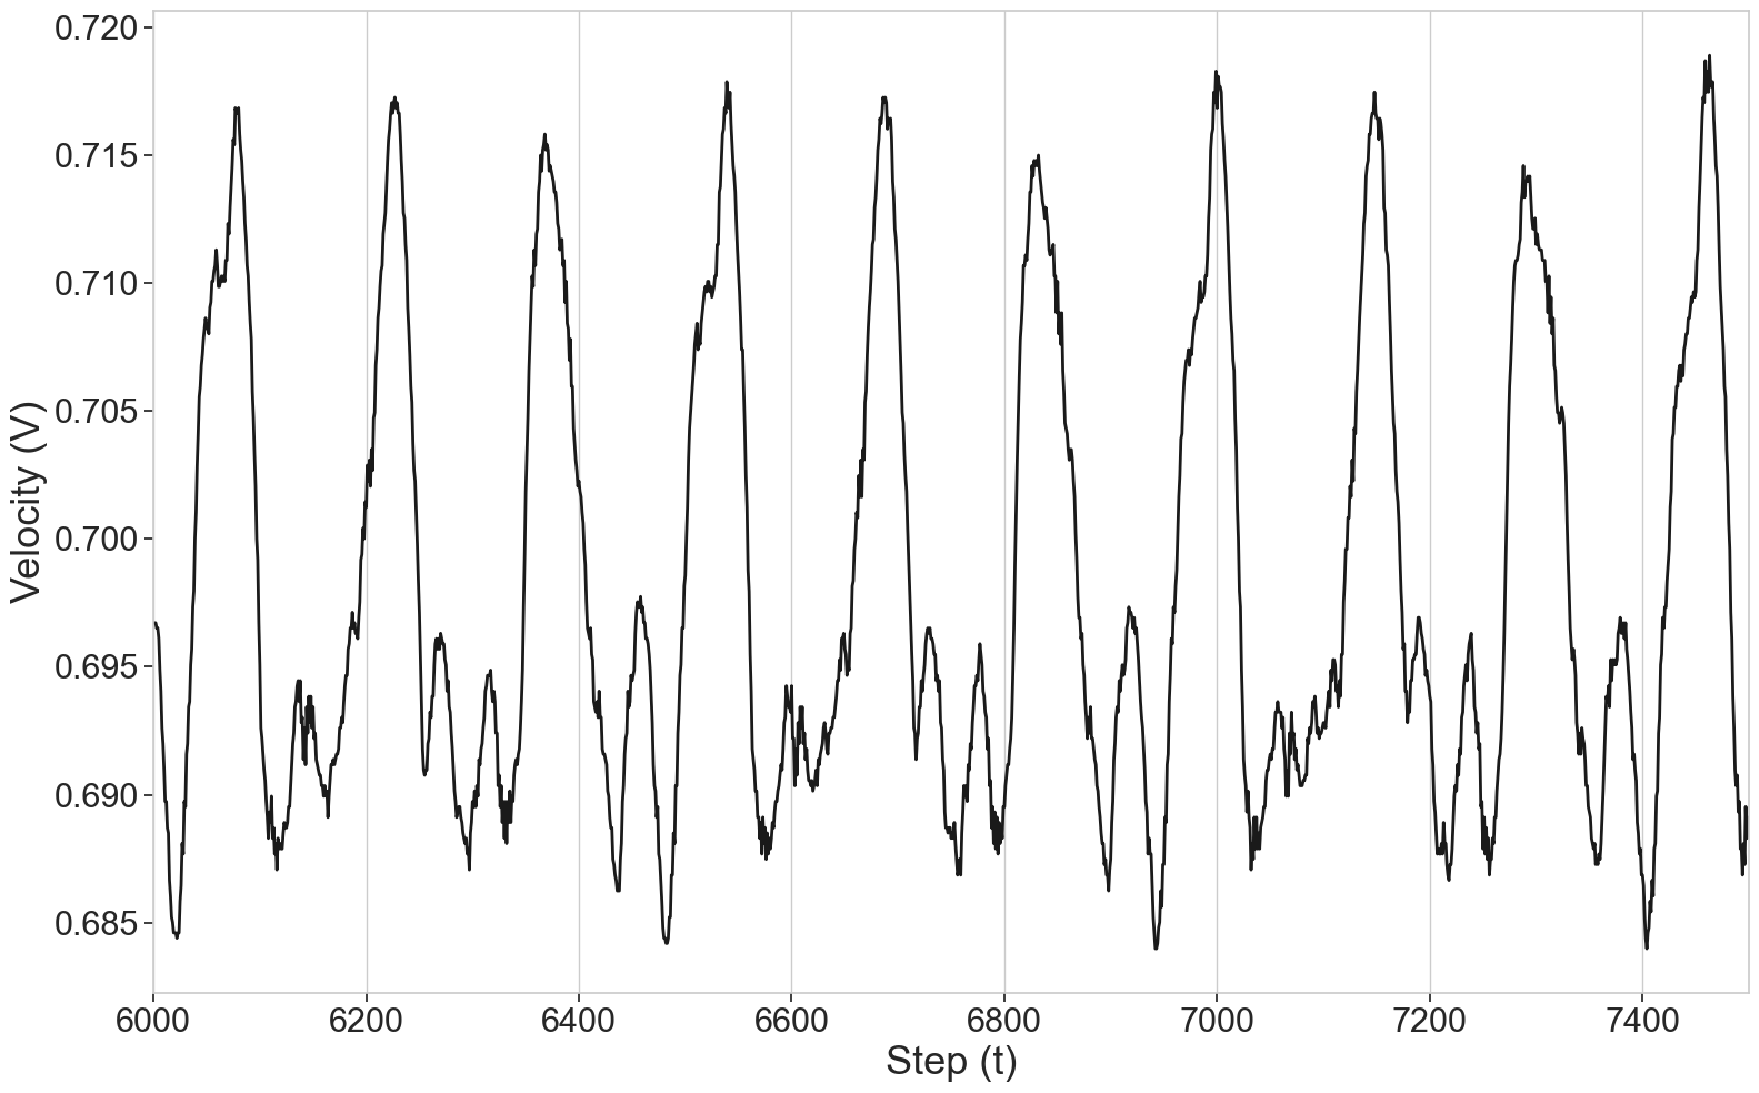
\includegraphics[width=\linewidth]{Images/Section 4/Experiment 3/Velocity_zoomed.pdf}
    \caption{A closer look at the velocity of the system at iterations $6,000 \rightarrow 7,500$.}
    \label{fig:Experiment-3.2}
\end{figure}

\begin{figure}[H]
    \centering
    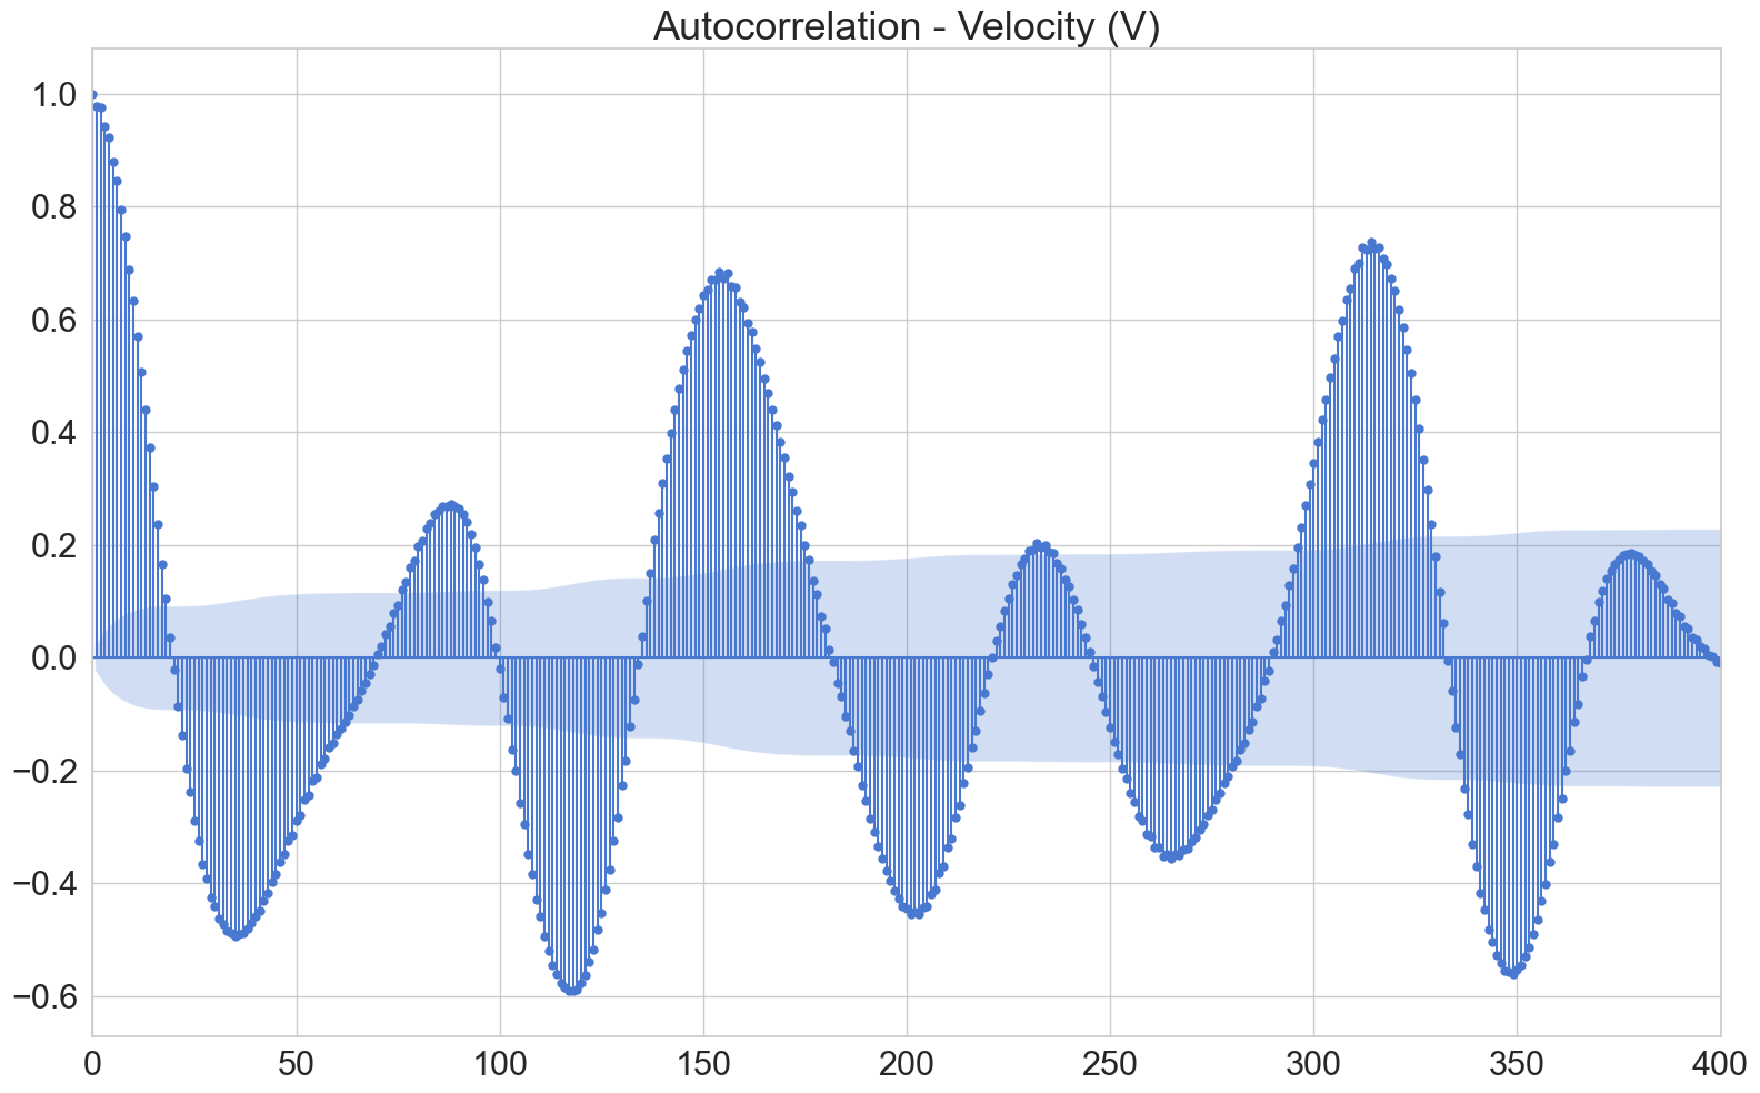
\includegraphics[width=\linewidth]{Images/Section 4/Experiment 3/Autocorrelation.pdf}
    \caption{Plotting the autocorrelation of the velocity of the system in an attempt to illustrate the periodic nature of the intermediate state that the system self-organized to.}
    \label{fig:Experiment-3.3}
\end{figure}


\begin{figure}[H]
        \myfloatalign
        \subfloat[Time step: 6250.]
        {
                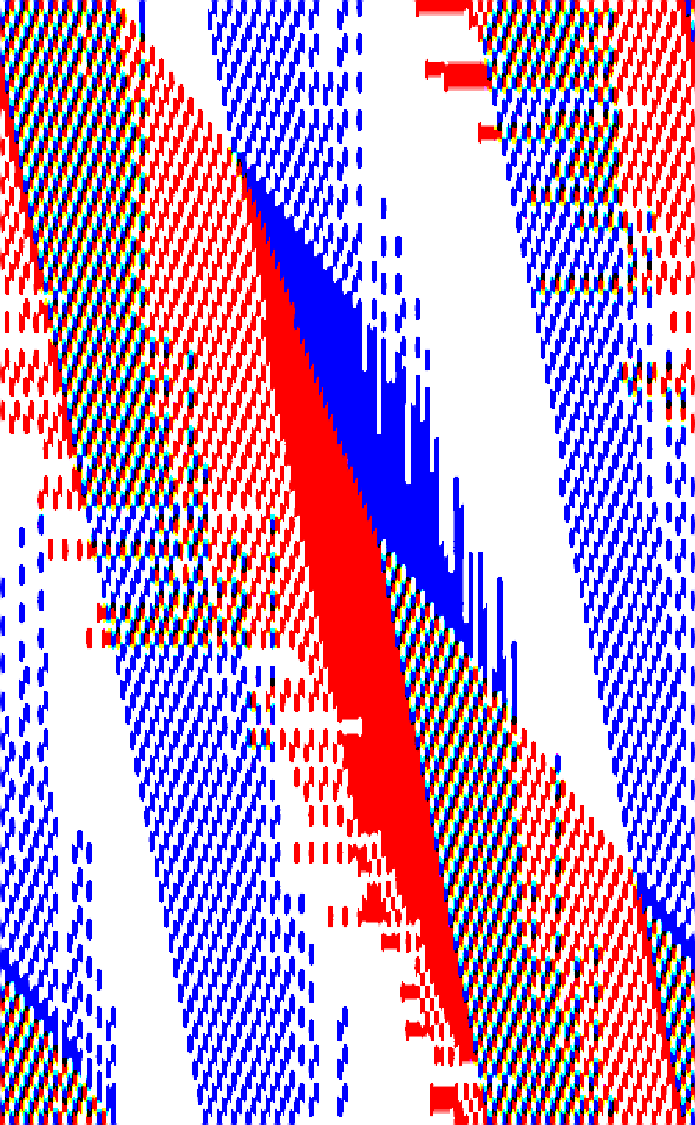
\includegraphics[width=0.45\linewidth]{Images/Section 4/Experiment 3/Simulation_step_6250.pdf}
        } \quad
        \subfloat[Time step: 6415.]
        {
                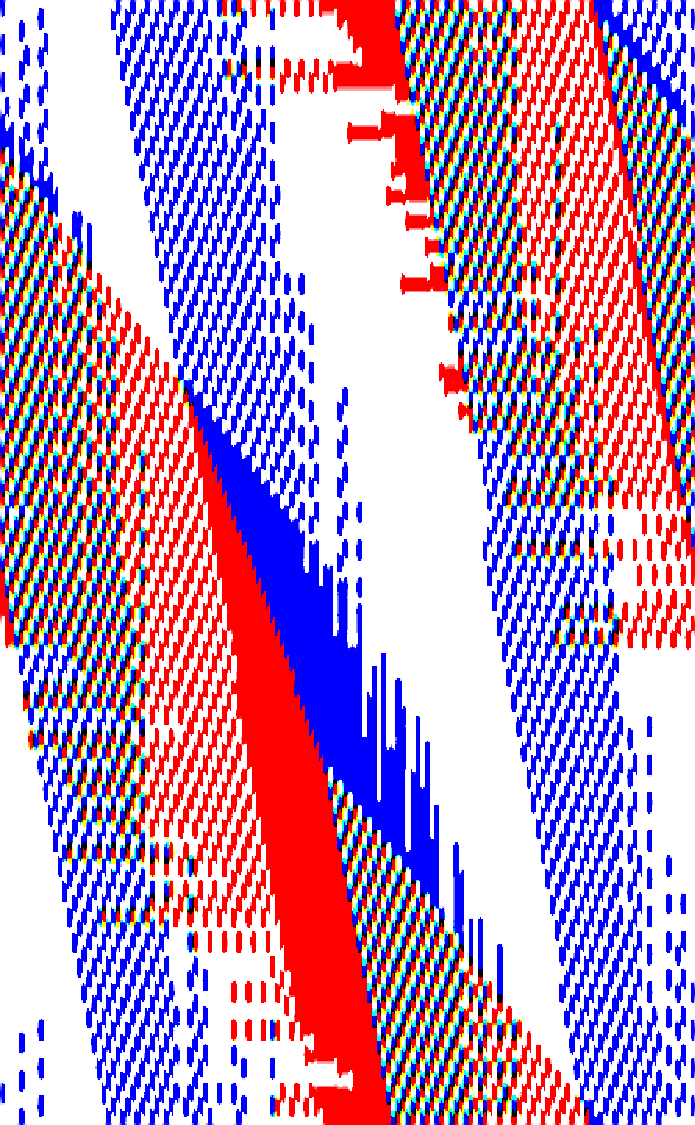
\includegraphics[width=0.45\linewidth]{Images/Section 4/Experiment 3/Simulation_step_6415.pdf}
        } \quad
        \caption{A snapshot of our system at 2 separate iterations (165 iterations apart) illustrating the intermediate phase characterized by arrangements of traffic jams as well as smoothly flowing traffic.}
\end{figure}